\chapter[Prefixing-based Method for Asynchronous Communication]{Prefixing-based Method for Asynchronous
Communication}\label{prefixing}

In this Chapter  we propose a general encoding method based on
extending an additive error correction code with a prefix to
include immunity to multiple synchronization errors. The length of
the prefix scales as $O(\log n)$ where $n$ denotes the codeword
length. In the context of transmitting LDPC codes over channels
that introduce both additive and repetition errors, we also
provide a modified message passing algorithm suitable for decoding
LDPC codes with such a prefix. The complexity of the proposed
modified decoding is on the same order as of the traditional
message passing algorithm used to decode LDPC codes over AWGN
channels.
\section{Introduction}

Suppose that $C$ denotes the additive error correction code used
for transmission over an AWGN channel . Let $\mathbf{c}$ denote a
codeword in $C$, and let $n$ be the codeword length. A binary
string $\mathbf{p}$ of length $m$ is prepended to the codeword
$\mathbf{c}$ chosen for transmission, and the resulting string
$\mathbf{t}=[\mathbf{p}~ \mathbf{c}]$ is sent over the channel. We
assume that the channel is additive white gaussian noise (AWGN).
In addition, $r$, $r \leq s$ repetitions are introduced as a
consequence of imperfect timing recovery. As a result, the
receiver performs a decoding algorithm on a sequence of length
$n+m+s$, and its goal is to recover the original sequence
$\mathbf{c}$.


Having established several useful ancillary results in Section
\ref{aux}, we then describe in Section \ref{enc} how to construct
``target'' string $\mathbf{t}$ used for transmission based on the
codeword $\mathbf{c}$ and the desired repetition-error correction
capability. We show that, by judiciously applying the construction
in Section \ref{aux} and using the number-theoretic constructions
from the previous chapter, it is possible to achieve $m$ that is
only $O(\log n)$, such that the target string $\mathbf{t}$ is
immune to $s$ repetitions. A decoding algorithm appropriate for
channels with $s$ repetitions and substitution errors based on
using LDPC codes is developed in Section \ref{dec}.

\section{Auxiliary results}\label{aux}
We now prove some auxiliary results which will be used in the
following section on encoding. Consider a prime number $P$.
Suppose that for a residue $z \mod P$ there exists $x$ such that
$x^i \equiv z \mod P$. We then say that $z$ is the $i$th power
residue. If the given integer $i$ satisfies $i |(P-1)$, then in
the residue set $\mod P$, there are $(P-1)/i$ $i$th power
residues, each having $i$ distinct $i$th power
roots~\cite{apostol}. Let $[x]_P$ indicate the residue mod $P$
congruent to $x$ .

\begin{lemma}\label{generates} For an integer $P$, each residue $r$ mod $P$ can be expressed as a
sum of a subset of elements of the set
$T_{z,P}=\{[z]_P,[2z]_P,[2^2z]_P,...,[2^{G}z]_P\}$ where
$G=\lfloor \log_2 P \rfloor $, $z$ is an arbitrary non zero
residue mod $P$.
\end{lemma}

\noindent \textit{Proof:} Observe that
$T_{1,P}=\{1,2,2^2,...,2^{G}\}$. We first show that each residue
$r$ mod $P$ can be expressed as a sum of a subset of elements of
the set $T_{1,P}$. Note that each residue $i$, $0 \leq i \leq
2^G-1$ (mod $P$) can be expressed as a sum of a subset, call it
$Q_i$, of the set $\{1,2,2^2,...,2^{G-1}\}$. Here $Q_0$ is the
empty set. Adding $2^G$ to the sum of each $Q_i$, for $0 \leq i
\leq 2^G-1$, generates the remaining residues $\{2^G,
2^G+1,...,P-1 \}$. As a result every residue mod $P$ can be
expressed as a sum of a subset of $T_{1,P}=\{1,2,2^2,...,2^{G}\}$.

Suppose there exists an element $r$ which cannot be expressed as a
sum of a subset of elements of $T_{z,P}$, for $z>1$, that is $r
\neq \sum_{i=0}^G \epsilon_i z 2^i \mod P$, for all choices of
$\{\epsilon_0,...,\epsilon_G\}$, $\epsilon_i \in \{0,1\}$. Let
$z^{-1}$ be the inverse element of $z$ under multiplication mod
$P$. Then the residue $r' = rz^{-1} \neq \sum_{i=0}^G \epsilon_i
2^i \mod P$, for all choices of $\{\epsilon_0,...,\epsilon_G\}$,
$\epsilon_i \in \{0,1\}$, which contradicts the result from the
previous paragraph.\hfill$\blacksquare$

\begin{lemma}\label{generates1} Suppose $P$ is a prime number such that $i|(P-1)$.
Let $z$ be an $i$th power residue. Suppose $x_{i,j}$ for $2 \leq j
\leq 2i-1$ are distinct $i$th power residues that are also
distinct from $z$ such that $2^{k}z \equiv x_{i,2k}+x_{i,2k+1}
\mod P$ for $1 \leq k \leq(i-1)$.

For such a prime $P$, each residue $r$ mod $P$ can be expressed as
a sum of a subset of elements of the set $L_{z,P}=
\bigcup_{j=1}^{2i-1} Y_j$ where $Y_j =\{[2^{il}x_{i,j}]_P| 0 \leq
l \leq \lfloor \frac{G-\lfloor \frac{l}{2}\rfloor}{i}\rfloor\}$
and $G=\lfloor \log_2 P \rfloor $.
\end{lemma}
\noindent \textit{Proof:} Follows immediately from the preceding
lemma by observing that we have in fact decomposed elements
$[2^{k}z]_P$ in the set $T_{z,P}$ for $k$ not a multiple of $i$
into a sum of two component elements such that all component
elements are distinct from one another and distinct from
$[2^kz]_P$ for $i|k$.\hfill$\blacksquare$



\begin{lemma}\label{sums} Suppose $P$ is a prime number such that $i|(P-1)$. Suppose the
equation $x^i\equiv a \mod P$ has a solution, $1 \leq a \leq P-1$.
Then the equation $x^i\equiv a \mod P$ has $i$ distinct solutions
\cite{apostol} and we may call them $x_1$ through $x_i$. The sum
$\sum_{k=1}^i x_k^j \equiv 0 \mod P$ for $1 \leq j \leq i-1$.
\end{lemma}
\noindent \textit{Proof:} Let us consider the equation $x^i \equiv
a \mod P$. Using Vieta's formulas and Newton's identities over
$GF(P)$ it follows that
 $\sum_{k=1}^i x_k^j \equiv 0 \mod P$ for $1 \leq j \leq
i-1$.\hfill$\blacksquare$

For a prime number $P$ for which $i|P-1$, and $i<P-1$, let
$Q_i(P)$ be the set of distinct $i$th power residues mod $P$, let
$N_i(P)$ be the set of distinct $i$th power non residues mod $P$.
We also state the following convenient result.
\begin{lemma}\label{sums1}
For a prime $P$ such that $i | (P-1)$, each residue $n \mod P$ can
be expressed as a sum of two distinct elements of $Q_i(P)$ in at
least $P/(2i^2)-\sqrt{P}/2-3$ ways.
\end{lemma}
\noindent \textit{Proof:} The result follows from Theorem II in
\cite{huavan:49} which states that over $GF(P)$ the equation
\begin{equation}\label{hua} x^i+y^i=a
\end{equation} where $x,y,a \in GF(P)$ and nonzero and $0 < i <P-1 $
has at least
$P-(i-1)^2\sqrt{P}-2(i-1)-2+\frac{1}{P}-\frac{1}{\sqrt{P}}$
solutions. Noting that $i$ distinct values of $x$ result in the
same $x^i$, accounting for the symmetry of $x$ and $y$, and
omitting the case $x^i=y^i$ we obtain a lower bound on the number
of solutions as $P/(2i^2)-\sqrt{P}/2-3$. \hfill$\blacksquare$

Equations of the type in (\ref{hua}) were also studied by Weil
\cite{weil:49}.

Given a positive integer $s$, suppose $lcm(2,3,..s) | (P-1)$ for
$P$ prime. Then, for each $i$, $1 \leq i \leq s$, in the residue
set $\mod P$, there are $\frac{P-1}{i}$ elements that are $i$th
power residues. For convenience, let $G = \lfloor \log_2(P)
\rfloor$.

For each $i$, $1 \leq i \leq s$ we will construct a specific
subset $V_i$ of the $i$th power residues $\mod P$ such that all
other residues can be expressed as a sum of a subset  of elements
of $V_i$, and such that $V_i$ has size that is logarithmic in $P$.
The set of the $i$th roots of the elements of the set $V_i$ will
be denoted $F_i$. Thus, $F_i$ will also have size logarithmic in
$P$. The elements of $M =\bigcup_{i=1}^s F_i$ will be reserved for
the indices of bins of zeros of the prefix string $\mathbf{p}$ in
the transformed domain. Note that $M$ also has size that is
logarithmic in $P$, and thus the length of the prefix is also
logarithmic in $P$. The sets $V_i$ will serve to satisfy the $i$th
congruency constraint of the type given in~\eqref{exten2} for the
string $\mathbf{\tilde{t}}$, as further described in the Section
on encoding.

In the remainder of this section we will first show how to
construct sets $V_i$, and then we will provide the proof that it
is possible to construct sets $V_i$ with all distinct elements as
well as  sets $F_i$ that have distinct elements and are non
intersecting, for $P$ large enough. We will also provide a proof
that for a given integer $n$, for $n$ large enough, there exists a
prime $P$ for which we can construct non intersecting sets $F_i$
containing distinct elements, where the prime $P$ lies in an
interval that linearly depends on $n$. Combined with the encoding
method described in the next Section we will therefore have
constructed a prefix whose length is logarithmic in $n$ such that
the overall string (prefix plus a codeword) in the transformed
domain satisfies equations of congruential type given
in~\eqref{exten2}, for which we have already proved in the
previous Chapter that are sufficient for the immunity to $s$
repetition errors.


By Lemma~\ref{sums}, for a prime $P$ such that $i| (P-1)$ it is
sufficient that $P/(2i^2)-\sqrt{P}/2-3>0$ for a nonzero residue
$\mod P$ to be expressed as a sum of two distinct $i$th power
residues. We thus consider a prime number $P$ such that $i|(P-1)$
for the given positive integer $i$ and such that
$P>i^2(\sqrt{P}-6)$.

We now continue with the introduction of some convenient notation.
For $z_i$ an $i$th power residue define the set $A_{i,1}(z_i)$ to
be
\begin{eqnarray}\label{azi1}A_{i,1}(z_i)=\{[2^{ik}z_i]_P | 0 \leq k \leq
\lfloor\frac{G}{i} \rfloor \}~.\end{eqnarray} Let $x_{i,2}$ and
$x_{i,3}$ be distinct $i$th power residues such that
$x_{i,2}+x_{i,3} \equiv 2z_i \mod P$ (possible by
Lemma~\ref{sums1} since $P>i^2(\sqrt{P}-6)$). These two power
residues generate sets $A_{i,2}(x_{i,2})$ and  $A_{i,3}(x_{i,3})$
where
\begin{eqnarray}\label{azi2} A_{i,2}(x_{i,2}) =\{ [2^{ik}x_{i,2}]_P| 0 \leq k \leq \lfloor
\frac{G-1}{i} \rfloor \} \text{ and }\\
\label{azi3}A_{i,3}(x_{i,3}) =\{ [2^{ik}x_{i,3}]_P| 0 \leq k \leq
\lfloor \frac{G-1}{i} \rfloor \}~.\end{eqnarray}

Likewise, for each $2^lz_i$ for $2 \leq l \leq i-1$ let $x_{i,2l}$
and $x_{i,2l+1}$ be distinct $i$th power residues such that
$x_{i,2l} + x_{i,2l+1} \equiv 2^lz_i \mod P$ (possible by
Lemma~\ref{sums1}). These residues generate sets
$A_{i,2l}(x_{i,2l})$ and  $A_{i,2l+1}(x_{i,2l+1})$ where
\begin{eqnarray}\label{azi2l}
A_{i,2l}(x_{i,2l}) =\{ [2^{ik}x_{i,2l}]_P| 0 \leq k \leq \lfloor
\frac{G-\lfloor \frac{l}{2} \rfloor}{i} \rfloor \} \text{ and }\\
\label{azi2l}A_{i,2l+1}(x_{i,2l+1}) =\{ [2^{ik}x_{i,2l+1}]_P| 0
\leq k \leq \lfloor \frac{G-\lfloor \frac{l}{2} \rfloor}{i}
\rfloor \}.\end{eqnarray}

By introducing sets $A_{i,j}(x_{i,j})$ we have effectively
decomposed all residues of the type $[2^lz_i]_P$ for which $i$ is
not a divisor of $l$ into a sum of two $i$th power residues,
namely $x_{i,2l}$ and $x_{i,2l+1}$. For each set
$A_{i,j}(x_{i,j})$, $1 \leq j \leq 2i-1$, we let
$B_{i,j}(x_{i,j})$ be the set of all $i$th power roots of elements
of $A_{i,j}(x_{i,j})$. First note that all elements in
$A_{i,j}(x_{i,j})$ are $i$th power residues by construction.
Moreover, they are all distinct since  $2^{ij_1} \neq 2^{ij_2}
\mod P$ for $1 \leq j_1,j_2 \leq \lfloor
\frac{G-\lfloor\frac{j}{2} \rfloor}{i} \rfloor$ for $j_1\neq j_2$
implies $x_{i,j}2^{ij_1} \neq x_{i,j}2^{ij_2} \mod P$. Thus,
$|A_{ij}(x_{i,j})|=\lfloor \frac{G-\lfloor \frac{j}{2}\rfloor}{i}
\rfloor+1$ and since the $i$th power roots of distinct $i$th power
residues are themselves distinct,
$|B_{ij}(x_{i,j})|=i\left(\lfloor \frac{G-\lfloor
\frac{j}{2}\rfloor}{i} \rfloor+1\right)$.



The following lemma proves that it is possible to construct
subsets $A_{ij}(x_{i,j})$, and subsets $B_{ij}(x_{i,j})$ from
them, of the set of residues $\mod P$ for $P$ prime that satisfies
$lcm(2,3,...s) | (P-1)$ for a given positive integer $s$, provided
that $P$ is large enough such that for fixed $i$ the subsets
$A_{ij}(x_{i,j})$ are disjoint, and such that \emph{all} subsets
$B_{ij}(x_{i,j})$ for $1 \leq i \leq s$, $1 \leq j \leq 2i-1$ are
also disjoint. Let $W_i$ denote the number of ways a residue $\mod
P$ can be expressed as a sum of two distinct non zero $i$th power
residues $\mod P$. A lower bound on $W_i$ is given in
Lemma~\ref{sums}.
\begin{lemma}\label{lemmaw} For a given integer $s$, suppose a prime number $P$ satisfies $lcm(2,3,...s) |
(P-1)$. Let $G =\lfloor \log_2{P}\rfloor$. If $P-1 >
(G+s)(G+s-1)(s-1)^2$ and $W_i
> 2i(G+i)(G+i-1)$, for each $i$ in the range $2 \leq i \leq
s$, there exist subsets $A_{ij}(x_{i,j})$ and $B_{ij}(x_{i,j})$
 such that all $B_{ij}(x_{i,j})$ are disjoint for $1 \leq i \leq
s$ and $1 \leq j \leq 2i-1$.
\end{lemma}
\noindent \textit{Proof:} We inductively build the sets
$A_{ij}(x_{i,j})$ and $B_{ij}(x_{i,j})$ for $1 \leq i \leq s$ and
$1 \leq j \leq 2i-1$, starting with the level $i=1$. We then
increment $i$ by one to reach the next $A_{ij}(x_{i,j})$ and
$B_{ij}(x_{i,j})$ while making sure the sets $B_{ij}(x_{i,j})$ at
the current level are disjoint with one another and with all
previously constructed sets at lower levels.

Consider $i=1$. Let $z_1$ be an arbitrary residue$~\mod P$, and
let \[A_{1,1}(z_1)=\{[2^{k}z_1]_P | 0 \leq k \leq G \}.\] For
notational convenience let $x_{1,1}=z_1$ and
$y_{1,1}^{(1)}=x_{1,1}$. Here $B_{1,1}(x_{1,1})$ is simply
$A_{1,1}(z_1)$ for $i=1$. All elements in $B_{1,1}(x_{1,1})$ are
distinct and $|B_{1,1}(x_{1,1})| =(G+1)$. If $s=1$, we are done,
as we did not even appeal to $W_1$ nor the condition on the lower
bound on $P-1$ (it is simply $P-1>0$).

If $s>2$, let us consider $i=2$. Consider quadratic residues
$x_{2,1}$, $x_{2,2}$ and $x_{2,3}$. Let  their respective distinct
quadratic roots be $y_{2,1}^{(1)}$, $y_{2,1}^{(2)}$ (so that
$(y_{2,1}^{(1)})^2 \equiv (y_{2,1}^{(2)})^2 \equiv x_{2,1} \mod
P$), $y_{2,2}^{(1)}$, $y_{2,2}^{(2)}$ (so that $(y_{2,2}^{(1)})^2
\equiv (y_{2,2}^{(2)})^2 \equiv x_{2,2} \mod P$) and
$y_{2,3}^{(1)}$, $y_{2,3}^{(2)}$ (so that $(y_{2,3}^{(1)})^2
\equiv (y_{2,3}^{(2)})^2 \equiv x_{2,3} \mod P$). These quadratic
residues give rise to sets
\begin{eqnarray}
A_{2,1}(x_{2,1})&=&\{ [2^{2k}x_{2,1}]_P | 0 \leq k \leq \lfloor
\frac{G}{2} \rfloor\},\\ A_{2,2}(x_{2,2})&=& \{ [2^{2k}x_{2,2}]_P
| 0
\leq k \leq \lfloor \frac{G-1}{2} \rfloor\} \text{ and},\\
A_{2,3}(x_{2,3})&=& \{ [2^{2k}x_{2,2}]_P | 0 \leq k \leq \lfloor
\frac{G-1}{2} \rfloor\}~.
\end{eqnarray}
Quadratic roots of elements of sets $A_{2,1}(x_{2,1})$,
$A_{2,2}(x_{2,2})$ and $A_{2,3}(x_{2,3})$ give rise to sets
$B_{2,1}(x_{2,1})$, $B_{2,2}(x_{2,2})$ and $B_{2,3}(x_{2,3})$,
\begin{eqnarray}
B_{2,1}(x_{2,1})&=&\{[2^ky_{2,1}^{(t)}]_P | 1 \leq t \leq 2, 0
\leq k
\leq \lfloor \frac{G}{2}\rfloor\},\\
B_{2,2}(x_{2,2})&=&\{[2^ky_{2,2}^{(t)}]_P | 1 \leq t \leq 2, 0
\leq k
\leq \lfloor \frac{G-1}{2}\rfloor\}, \text{ and}\\
B_{2,3}(x_{2,3})&=&\{[2^ky_{2,3}^{(t)}]_P | 1 \leq t \leq 2, 0
\leq k \leq \lfloor \frac{G-1}{2}\rfloor\}~.
\end{eqnarray}


Having fixed the set $B_{1,1}(x_1)$ based on the earlier selection
of the residue $x_{1,1} (=z_1)$, we want to show that it is
possible to find quadratic residues $x_{2,1}$, $x_{2,2}$ and
$x_{2,3}$ such that $x_{2,2} + x_{2,3} \equiv 2x_{2,1} \mod P$ and
such that the resulting sets $B_{1,1}(x_1)$, $B_{2,1}(x_{2,1})$,
$B_{2,2}(x_{2,2})$ and $B_{2,3}(x_{2,3})$ are all disjoint.

In particular we require that $x_{2,1}$ is a quadratic
residue$~\mod P$ (there are $(P-1)/2$ quadratic residues) with a
property that the set $B_{2,1}(x_{2,1})$ is disjoint with
$B_{1,1}(x_{1,1})$. That is we require \[y_{2,1}^{(1)}2^k \neq
y_{1,1}^{(1)} 2^l \mod P \] and
\[y_{2,1}^{(2)}2^k \neq y_{1,1}^{(1)} 2^l \mod P \] for $0 \leq k \leq \lfloor
\frac{G}{2} \rfloor$ and $0 \leq l \leq G$. By squaring the
expressions, these two conditions can be combined into
\begin{equation}\label{x21}x_{2,1}2^{2k} \neq (y_{1,1}^{(1)})^2 2^{2l} \mod P \end{equation}for $0
\leq k \leq \lfloor \frac{G}{2} \rfloor$ and $0 \leq l \leq G$.
For the already chosen $y_{1,1}^{(1)}(=x_{1,1}=z_1)$ at most
$(G+1)(\lfloor \frac{G}{2} \rfloor+1)$ candidate quadratic
residues out of total $(P-1)/2$ quadratic residues violate
~\eqref{x21}. Since $\frac{P-1}{2} > \frac{(G+1)(G+2)}{2} \geq
(G+1)(\lfloor \frac{G}{2} \rfloor+1)$ by assumption (the function
$(G+i)(G+i-1)(i-1)^2$ is strictly increasing for positive $i$, $2
\leq i \leq s$, the condition $P-1> (G+s)(G+s-1)(s-1)^2$ implies
$P-1>(G+2)(G+1)$), such $x_{2,1}$ exists.

Fix $x_{2,1}$ such that \eqref{x21} holds. Having chosen such
$x_{2,1}$, we now look for $x_{2,2}$ and $x_{2,3}$ quadratic
residues that satisfy $x_{2,2}+x_{2,3} \equiv 2x_{2,1} \mod P$. We
require that $B_{2,2}(x_{2,2})$ be disjoint with both
$B_{1,1}(x_{1,1})$ and $B_{2,1}(x_{2,1})$ so that
\begin{eqnarray*}
y_{2,2}^{(1)}2^{k_3} \neq y_{1,1}^{(1)} 2^{k_1} \mod P, \\
y_{2,2}^{(2)}2^{k_3} \neq y_{1,1}^{(1)} 2^{k_1} \mod P,  \\
y_{2,2}^{(1)}2^{k_3} \neq y_{2,1}^{(1)} 2^{k_2} \mod P, \\
y_{2,2}^{(2)}2^{k_3} \neq y_{2,1}^{(1)} 2^{k_2} \mod P,  \\
y_{2,2}^{(1)}2^{k_3} \neq y_{2,1}^{(2)} 2^{k_2} \mod P, \\
y_{2,2}^{(2)}2^{k_3} \neq y_{2,1}^{(2)} 2^{k_2} \mod P,
\end{eqnarray*}
where $0 \leq k_1 \leq G$, $0 \leq k_2 \leq \lfloor \frac{G}{2}
\rfloor$ and $0 \leq k_3 \leq \lfloor\frac{G-1}{2} \rfloor$.

Alternatively,
\begin{equation}\label{eqx22}\begin{array}{cccc}
x_{2,2}2^{2k_3} &\neq& (y_{1,1}^{(1)})^2 2^{2k_1} &\mod P, \\
x_{2,2}2^{2k_3} &\neq& x_{2,1} 2^{2k_2} &\mod P,
\end{array}\end{equation}
where $0 \leq k_1 \leq G$, $0 \leq k_2 \leq \lfloor \frac{G}{2}
\rfloor$ and $0 \leq k_3 \leq \lfloor\frac{G-1}{2} \rfloor$.

Likewise, we require that $B_{2,3}(x_{2,3})$ be disjoint with both
 of  $B_{1,1}(x_{1,1})$, $B_{2,1}(x_{2,1})$ as well as with
$B_{2,2}(x_{2,2})$, so that
\begin{equation}\label{eqx23}\begin{array}{cccc}
x_{2,3}2^{2k_3} &\neq& (y_{1,1}^{(1)})^2 2^{2k_1} &\mod P, \\
x_{2,3}2^{2k_3} &\neq& x_{2,1} 2^{2k_2} &\mod P, \\
x_{2,3}2^{2k_3} &\neq& x_{2,2} 2^{2k_3} &\mod P, \\
\end{array}\end{equation}
where $0 \leq k_1 \leq G$, $0 \leq k_2 \leq \lfloor \frac{G}{2}
\rfloor$ and $0 \leq k_3 \leq \lfloor\frac{G-1}{2} \rfloor$. For
already chosen values of $x_{2,1}$ and $y_{1,1}$ at most $N_2=
2\left[ \left(\lfloor \frac{G}{2} \rfloor +1 \right)\left(\lfloor
\frac{G-1}{2} \rfloor +1 \right)+ \left( G+1 \right)\left(\lfloor
\frac{G-1}{2} \rfloor +1 \right)\right]+\left( \lfloor
\frac{G-1}{2} \rfloor +1 \right)^2  $ choices for $x_{2,2}$ and
$x_{2,3}$ violate~\eqref{eqx22} and ~\eqref{eqx23}.

We thus require that $W_2$ be strictly larger than $N_2$. Dropping
floor operations it is sufficient that $W_2 > \frac{(G+1)(G+2)}{2}
+ \frac{5(G+1)^2}{4}$. Further  simplification yields that
\begin{equation}
W_2 > \frac{7(G+1)(G+2)}{4}
\end{equation}
is sufficient to ensure that there exist $x_{2,2}$, $x_{2,3}$ that
make the respective sets disjoint. Note that this last condition
follows from the requirement in the statement of the Lemma for
$i=2$, namely that $W_2 > 4(G+1)(G+2)$. If $s=2$ we are done, else
we consider $i=3$. Before considering general level $i$ let us
present the $i=3$ case.

For $i=3$ we seek distinct cubic residues $x_{3,1}$, $x_{3,2}$,
$x_{3,3}$, $x_{3,4}$ and $x_{3,5}$ with the property that
$x_{3,2}+ x_{3,3} \equiv 2x_{3,1} \mod P$ and $x_{3,4}+ x_{3,5}
\equiv 2^2x_{3,1} \mod P$, and such that the respective sets
$B_{3,j}(x_{3,j})$ for $1 \leq j \leq 5$ generated from the cubic
roots of these residues are disjoint and are disjoint with
previously constructed sets $B_{1,1}(x_{1,1})$,
$B_{2,1}(x_{2,1})$, $B_{2,2}(x_{2,2})$ and $B_{2,3}(x_{2,3})$.


We start with $x_{3,1}$ a cubic residue$~\mod P$ (there are
$(P-1)/3$ quadratic residues) with a property that the set
$B_{3,1}(x_{3,1})$ is disjoint with each of $B_{1,1}(x_{1,1})$
$B_{2,1}(x_{2,1})$, $B_{2,2}(x_{2,2})$ and $B_{2,3}(x_{2,3})$.
That is, after raising the elements of these sets to the third
power, we require
\begin{equation}\label{eqx31}\begin{array}{cccc}
x_{3,1}2^{3k_4} &\neq& (y_{1,1}^{(1)})^3 2^{3k_1} &\mod P, \\
x_{3,1}2^{3k_4} &\neq& (y_{2,1}^{(1)})^3 2^{3k_2} &\mod P, \\
x_{3,1}2^{3k_4} &\neq& (y_{2,1}^{(2)})^3 2^{3k_2} &\mod P, \\
x_{3,1}2^{3k_4} &\neq& (y_{2,2}^{(1)})^3 2^{3k_3} &\mod P, \\
x_{3,1}2^{3k_4} &\neq& (y_{2,2}^{(2)})^3 2^{3k_3} &\mod P, \\
x_{3,1}2^{3k_4} &\neq& (y_{2,3}^{(1)})^3 2^{3k_3} &\mod P, \\
x_{3,1}2^{3k_4} &\neq& (y_{2,3}^{(2)})^3 2^{3k_3} &\mod P, \\
\end{array}\end{equation}
where $0 \leq k_1 \leq G$, $0 \leq k_2 \leq \lfloor \frac{G}{2}
\rfloor$, $0 \leq k_3 \leq \lfloor\frac{G-1}{2} \rfloor$ and $0
\leq k_4 \leq \lfloor\frac{G}{3} \rfloor$.

For already chosen values of $x_{1,1}$ through $x_{2,3}$, which in
turn determine $y_{1,1}^{(1)}$ through $y_{2,3}^{(2)}$, the
condition in~\eqref{eqx31} prevents $N_3= \left(\lfloor
\frac{G}{3} \rfloor +1 \right)\left[ (G+1)+2\left(\lfloor
\frac{G}{2} \rfloor +1 \right) +4\left(\lfloor \frac{G-1}{2}
\rfloor +1 \right)\right]$ choices for $x_{3,1}$. Since there are
$\frac{P-1}{3}$ cubic residues, after simplifying and upper
bounding the expression for $N_3$, it follows that it is
sufficient that $\frac{P-1}{3}$ be strictly larger than
$\frac{4(G+2)(G+3)}{3}$. Note that this condition is implied by
the requirement that $P-1> (s-1)^2(G+s)(G+s-1)$ (again, since the
function $(i-1)^2(G+i)(G+i-1)$ is strictly increasing for positive
$i$).

Fix $x_{3,1}$ such that \eqref{eqx31} holds. Having chosen such
$x_{3,1}$, we now look for distinct $x_{3,2}$, $x_{3,3}$,
$x_{3,4}$, $x_{3,5}$ cubic residues that satisfy $x_{3,2}+x_{3,3}
\equiv 2x_{3,1} \mod P$ and $x_{3,4}+x_{3,5} \equiv 2^2x_{3,1}
\mod P$ that make all sets $B_{i,j}$, $1 \leq i \leq 3$, $1 \leq j
\leq 2i-1$ disjoint.

In order that residue $x_{3,2}$ generates set $B_{3,2}(x_{3,2})$
with the property that $B_{3,2}(x_{3,2})$ is disjoint with each of
$B_{1,1}(x_{1,1})$, $B_{2,1}(x_{2,1})$, $B_{2,2}(x_{2,2})$,
$B_{2,3}(x_{2,3})$ and $B_{3,1}(x_{3,1})$, we require that their
respective elements raised to the third power be distinct,
\begin{equation}\label{eqx32}\begin{array}{cccc}
x_{3,2}2^{3k_5} &\neq& (y_{1,1}^{(1)})^3 2^{3k_1} &\mod P, \\
x_{3,2}2^{3k_5} &\neq& (y_{2,1}^{(1)})^3 2^{3k_2} &\mod P, \\
x_{3,2}2^{3k_5} &\neq& (y_{2,1}^{(2)})^3 2^{3k_2} &\mod P, \\
x_{3,2}2^{3k_5} &\neq& (y_{2,2}^{(1)})^3 2^{3k_3} &\mod P, \\
x_{3,2}2^{3k_5} &\neq& (y_{2,2}^{(2)})^3 2^{3k_3} &\mod P, \\
x_{3,2}2^{3k_5} &\neq& (y_{2,3}^{(1)})^3 2^{3k_3} &\mod P, \\
x_{3,2}2^{3k_5} &\neq& (y_{2,3}^{(2)})^3 2^{3k_3} &\mod P, \\
x_{3,2}2^{3k_5} &\neq& x_{3,1} 2^{3k_4} &\mod P,
\end{array}\end{equation}
where $0 \leq k_1 \leq G$, $0 \leq k_2 \leq \lfloor \frac{G}{2}
\rfloor$, $0 \leq k_3 \leq \lfloor\frac{G-1}{2} \rfloor$, $0 \leq
k_4 \leq \lfloor\frac{G}{3} \rfloor$ and $0 \leq k_5 \leq
\lfloor\frac{G-1}{3} \rfloor$.

Likewise, we require that $B_{3,3}(x_{3,3})$ be disjoint with all
of  $B_{1,1}(x_{1,1})$, $B_{2,1}(x_{2,1})$, $B_{2,2}(x_{2,2})$,
$B_{2,3}(x_{2,3})$ $B_{3,1}(x_{3,1})$ and $B_{3,2}(x_{3,2})$, so
that
\begin{equation}\label{eqx33}\begin{array}{cccc}
x_{3,3}2^{3k_5} &\neq& (y_{1,1}^{(1)})^3 2^{3k_1} &\mod P, \\
x_{3,3}2^{3k_5} &\neq& (y_{2,1}^{(1)})^3 2^{3k_2} &\mod P, \\
x_{3,3}2^{3k_5} &\neq& (y_{2,1}^{(2)})^3 2^{3k_2} &\mod P, \\
x_{3,3}2^{3k_5} &\neq& (y_{2,2}^{(1)})^3 2^{3k_3} &\mod P, \\
x_{3,3}2^{3k_5} &\neq& (y_{2,2}^{(2)})^3 2^{3k_3} &\mod P, \\
x_{3,3}2^{3k_5} &\neq& (y_{2,3}^{(1)})^3 2^{3k_3} &\mod P, \\
x_{3,3}2^{3k_5} &\neq& (y_{2,3}^{(2)})^3 2^{3k_3} &\mod P, \\
x_{3,3}2^{3k_5} &\neq& x_{3,1} 2^{3k_4} &\mod P, \\
x_{3,3}2^{3k_5} &\neq& x_{3,2} 2^{3k_5} &\mod P,
\end{array}\end{equation}
where $0 \leq k_1 \leq G$, $0 \leq k_2 \leq \lfloor \frac{G}{2}
\rfloor$, $0 \leq k_3 \leq \lfloor\frac{G-1}{2} \rfloor$, $0 \leq
k_4 \leq \lfloor\frac{G}{3} \rfloor$ and $0 \leq k_5 \leq
\lfloor\frac{G-1}{3} \rfloor$.

From~\eqref{eqx32} and~\eqref{eqx33} it follows that at most
\begin{equation}\label{w31}\begin{array}{lll} 2 \left( \lfloor \frac{G-1}{3}\rfloor +1\right) \left[
(G+1)+2\left( \lfloor \frac{G}{2}\rfloor +1\right) +4\left(
\lfloor \frac{G-1}{2}\rfloor +1\right) + \left( \lfloor
\frac{G}{3}\rfloor +1\right)\right]+ \\\left( \lfloor
\frac{G-1}{3}\rfloor +1\right)^2.
\end{array}\end{equation}
candidate pairs $(x_{3,2},x_{3,3})$ do not make the respective
$B_{i,j}(x_{i,j})$ sets disjoint. After some simplification, it
follows that it is sufficient that
\begin{equation}\label{w311}
W_3 > 3 (G+2)(G+3)~,
\end{equation}
where $W_3$ is the number of ways a residue $\mod P$ can be
expressed as a sum of two different cubic residues. Similarly, the
cubic residues $x_{3,4}$ and $x_{3,5}$ for which the respective
disjoint $B_{i,j}(x_{i,j})$ sets  exist, provided that
\begin{equation}\label{w31a}\begin{array}{lll} W_3
> 2 \left( \lfloor \frac{G-2}{3}\rfloor +1\right)\left[
(G+1)+2\left( \lfloor \frac{G}{2}\rfloor +1\right) +4\left(
\lfloor \frac{G-1}{2}\rfloor +1\right)  +\left( \lfloor
\frac{G}{3}\rfloor
+1\right)+\left( \lfloor \frac{G-1}{3}\rfloor +1\right)\right]+\\
\left( \lfloor \frac{G-2}{3}\rfloor +1\right)^2.
\end{array}\end{equation} The extra term in ~\eqref{w31a} relative
to ~\eqref{w31} comes from the disjointness of the sets
$B_{3,4}(x_{3,4})$ and $B_{3,5}(x_{3,5})$.
 Some simplification of ~\eqref{w31a} yields
\begin{equation}\label{w312}
W_3 > \frac{31}{9} (G+2)(G+3)~,
\end{equation}
which subsumes the lower bound on $W_3$ given in ~\eqref{w311}.
Note that ~\eqref{w312} is implied by the condition in the
statement of the Lemma, namely $W_3 >6(G+2)(G+3)$.

We now inductively show the existence of appropriate $i$th power
residues and their sets, assuming that we have successfully
identified power residues at lower levels for which all the sets
$B_{k,j}(x_{k,j})$ for $1 \leq k <i$, $1 \leq j \leq 2k-1$ are
disjoint.

Consider $x_{i,1}$ an $i$th power residue$~\mod P$ (there are
$(P-1)/i$ such  residues) with a property that the set
$B_{i,1}(x_{i,1})$ is disjoint with all of $B_{k,j}(x_{k,j})$ for
$1 \leq k <i$, $1 \leq j \leq 2k-1$.

These  constraints on disjointness (the example of which is given
in~\eqref{x21} for $i=2$ and in ~\eqref{eqx31} for $i=3$) prevent
no more than $(\frac{G+i}{i})(\frac{G+k}{k})$ choices for
$x_{i,1}$  for each $y_{k,j}^{(t)}$ where $1 \leq k \leq i-1$, $1
\leq j \leq 2k-1$, and $1 \leq t \leq k$ (since
$|B_{i,1}(x_{x,1})|=\lfloor \frac{G}{i} \rfloor+1 \leq
\frac{G+i}{i}$, and $|B_{k,j}(x_{k,j})|=\lfloor \frac{G-\lfloor
\frac{j}{2}\rfloor}{k} \rfloor+1 \leq \frac{G+k}{k}$). Summing
over all choices it follows that at most
\begin{equation}\begin{array}{lll}{}& \left(\frac{G+i}{i}\right) \sum_{k=1}^{i-1}
(2k-1)k\left(\frac{G+k}{k}\right)\\\leq&
(G+i)\left(\frac{G+i-1}{i}\right) \sum_{k=1}^{i-1}
(2k-1)\\=&(G+i)\left(\frac{G+i-1}{i}\right)(i-1)^2
\end{array}\end{equation} $i$th power residues cannot be chosen for
$x_{i,1}$. We thus require
\begin{equation}\label{preq}
P-1 > (G+i)(G+i-1)(i-1)^2
\end{equation}
for each level $i$. Note that since the expression on the right
hand side of the inequality ~\eqref{preq} is an increasing
function of positive $i$, each subsequent level poses a lower
bound on $P$ that subsumes all previous ones. Since there are
$\frac{P-1}{i}$ $i$th power residues, it is thus sufficient to
have $P-1
> (G+s)(G+s-1)(s-1)^2$, as given in the statement of the Lemma.

Consider $x_{i,2}$ and $x_{i,3}$ as distinct $i$th power
residues$~\mod P$ that satisfy $x_{i,2}+ x_{i,3} \equiv 2x_{i,1}
\mod P$ for a previously chosen $x_{i,1}$. We require that
 $x_{i,2}$ and $x_{i,3}$ give rise to sets $B_{i,2}(x_{i,2})$ and
$B_{i,3}(x_{i,3})$ that are disjoint and that are disjoint with
each of $B_{k,j}(x_{k,j})$ for $1\leq k \leq i$, $1\leq j \leq
2k-1$ and with $B_{i,1}(x_{i,1})$. Constraints based on previously
encountered $y_{j,k}^{(t)}$ for $1\leq k \leq i$, $1\leq j \leq
2k-1$, $1 \leq t \leq k$ prevent at most
$(\frac{G+i-1}{i})(\frac{G+j}{j})$ choices for each of $x_{i,2}$
and $x_{i,3}$, for each $y_{j,k}^{(t)}$ (since
$|B_{i,2}(x_{i,2})|=|B_{i,3}(x_{i,3})|= \lfloor \frac{G-1}{i}
\rfloor+1 \leq \frac{G+i-1}{i}$, and $|B_{k,j}(x_{k,j})|=\lfloor
\frac{G-\lfloor \frac{j}{2}\rfloor}{k} \rfloor+1 \leq
\frac{G+k}{k}$). Combined with the restriction based on the
disjointness with $B_{i,1}(x_{i,1})$ and the requirement that
$B_{i,2}(x_{i,2})$ and $B_{i,3}(x_{i,3})$ be nonintersecting, it
follows that
\begin{equation}\begin{array}{lll} W_i>
2\left(\frac{G+i-1}{i}\right) \left[\sum_{k=1}^{i-1}
(2k-1)k(\frac{G+k}{k})+\left( \frac{G+i}{i}\right)\right]+\left(
\frac{G-i+1}{i}\right)^2
\end{array}\end{equation}
is sufficient for the pair $(x_{i,2},x_{i,3})$ to exist.

Likewise, for  $x_{i,2l}$ and $x_{i,2l+1}$ as distinct $i$th power
residue$~\mod P$ that satisfy $x_{i,2l}+ x_{i,2l+1} \equiv
2^lx_{i,1} \mod P$, that give rise to disjoint sets
$B_{i,2l}(x_{i,2l})$ and $B_{i,2l+1}(x_{i,2l+1})$ that are also
disjoint from all previously constructed set $B_{k,j}$, we require
\begin{equation}\label{eqwi}\begin{array}{lll} W_i>
2(\frac{G+i-1}{i}) \left[\sum_{k=1}^{i-1}
(2k-1)k(\frac{G+k}{k})+(2l-1)\left(
\frac{G+i}{i}\right)\right]+\left( \frac{G-i+1}{i}+1\right)^2
\end{array}\end{equation}
for the pair $(x_{i,2l},x_{i,2l+1})$ to exist. Since at each level
$i$ we construct $i-1$ pairs $x_{i,2l}$ and $x_{i,2l+1}$, and
since the right hand side of~\eqref{eqwi} is an increasing
function of $l$, it is sufficient to upper bound the expression in
~\eqref{eqwi} for $l=i-1$. Some simplification yields
\begin{equation}\begin{array}{lll} W_i>
(G+i)(G+i-1)\frac{2i^3-4i^2+6i-5}{i^2}
\end{array}\end{equation}
as a sufficient condition for the disjoint sets $B_{i,j}(x_{i,j})$
to exist that all also disjoint with all sets $B_{k,l}(x_{k,l})$
for $k<i$.

Further simplifying the last inequality, it is sufficient that
\begin{equation}\begin{array}{lll} W_i>
2i(G+i)(G+i-1)
\end{array}\end{equation}
to make the these sets disjoint. We have thus demonstrated that
with appropriate lower bounds on $P$ and $W_i$'s, it is possible
to construct disjoint sets $B_{i,j}(x_{i,j})$.
 \hfill$\blacksquare$

Note that all residues$~\mod P$ can be expressed as sum of a
subset of elements of $V_i \asn
\bigcup_{j=1}^{2i-1}A_{ij}(x_{i,j})$ by Lemma~\ref{generates1} for
each $i$, $1\leq i \leq s$. Also note that $|V_i|$ scales as
$\log_2(P)$. For $F_i \asn \bigcup_{j=1}^{2i-1}B_{ij}(x_{i,j})$,
 $|F_i|$ also scales as
$\log_2(P)$.

We now discuss how large prime $P$ needs to be so that the
conditions of Lemma~\ref{lemmaw} hold. Namely we require
\begin{equation}\label{ne1}
P-1> (s-1)^2(G+s)(G+s-1) \end{equation} and
\begin{equation}\label{ne2}W_i>2i(G+i)(G+i-1) \text{ for }1 \leq i \leq s~. \end{equation} Using
Lemma~\ref{sums1} it follows that it is sufficient that
\begin{equation}\label{condp}
P > 4s^3(G+s)(G+s-1)+s^2\sqrt{P}+6s^2~,
\end{equation}
for both~\eqref{ne1} and~\eqref{ne2} to hold. This expression
certainly holds as $P\rightarrow \infty$, and for the finite
values of $P$ we (loosely) have that
\begin{eqnarray*}
P>10^3 \text{ for } s=1, \\P>10^4 \text{ for } s=2, \\P>10^5
\text{ for } s=3,\\ P>10^6 \text{ for } s=4,\\P>10^6 \text{ for }
s=5.
\end{eqnarray*}

 For a given large enough integer $n$, we now show that
there exists a prime number $P$ that satisfies~\eqref{condp}
(which holds for $P$ large enough) and for which $lcm(2,3,...,s) |
(P-1)$ such that $P$ lies in an interval that is linear in $n$.
Since the elements of $M \asn \bigcup_{i=1}^s F_i$ are to be
reserved for the indices of bins of zeros of the prefix in the
transformed domain we also require that $P-n > |M|$, since the
total number of bins of zeros to be used is at most $n$ (from the
codeword) + $|M|$ (from the prefix), and each bin receives a
distinct index. Since $F_i= \cup_{j=1}^{2i-1} B_{i,j}(x_{i,j})$
and $|B_{i,j}(x_{i,j})|$ =$i\left( \lfloor \frac{G-\lfloor
\frac{j}{2}\rfloor}{i}\rfloor+1\right)$ $\leq \frac{G+i}{i}$, it
follows that \begin{equation}\label{eqM} |M| \leq \sum_{i=1}^s
i(2i-1)\frac{G+i}{i} \leq (G+s) \sum_{i=1}^s (2i-1)
=(G+s)(s)^2\end{equation} yielding a sufficient requirement
\begin{equation}\label{condpn}P>n+(s-1)^2(\log_2(P)+s)~.
\end{equation}

For given integers $n$ and $s$ ($n$ is typically large and $s$ is
small), we essentially need to show that there exists a prime $P$
for which $k \asn lcm(2,3,...,s) | (P-1)$ and $P \in (c_1n,c_2n)$
(here $c_1$ and $c_2$ are positive numbers) and such that $P$
satisfies~\eqref{condp} and~\eqref{condpn}.

For the asymptotic regime as $n \rightarrow \infty$ we recall the
prime number theorem for arithmetic progression \cite{sopro} which
states that
\begin{equation}
\pi(n,k,1) \sim \frac{1}{\phi(k)} \frac{n}{\log(n)}~,
\end{equation}
where $\pi(n,k,1)$ denotes the number of primes $\leq n$ that are
congruent to $1 \mod k$, and $\phi(k)$ is the Euler function and
represents the number of integers $\leq k$ that are relatively
prime with $k$. As $n \rightarrow \infty$, we may let $c_1 \asn 2$
and $c_2 \asn 4$, so that
\begin{equation}
\frac{\pi(4n,k,1)}{\pi(2n,k,1)} \sim 2~,
\end{equation}
and thus there exists a prime $P$, $k | (P-1)$ in the interval
that is linear in $n$. Clearly, as $n \rightarrow \infty$, such
$P$ also satisfies ~\eqref{condp} and~\eqref{condpn}.



For finite (but possibly very large) values of $n$ and certain
small $s$ we appeal to results by Ramare and Rumely
\cite{rrumely}. The number-theoretic function $\theta(x;k,l)$ is
usually defined as
\[\theta(x;k,l)=\sum_{p \text{ prime }, p \equiv l \mod k, p
\leq x} \ln p~.\]

To show that there exists a prime $P$ in $(c_1n,c_2n)$ for which
$lcm(2,3,...,s) | (P-1)$  it is sufficient to have
\begin{equation} \theta(c_2n;k,1)> \theta(c_1n;k,1)~,\end{equation}
where $k=lcm(2,3,...,s)$.

Theorem 2 in \cite{rrumely} states that $|\theta(x;k,1)
-\frac{x}{\phi(x)}| \leq 2.072 \sqrt{x}$ for all $x \leq 10 ^{10}$
for $k$ given in Table I of \cite{rrumely}. For larger $x$,
Theorem 1 in \cite{rrumely}, provides the bounds of the type
\begin{equation}
(1-\varepsilon)\frac{x}{\phi(x)} \leq \theta(x;k,l) \leq
(1+\varepsilon)\frac{x}{\phi(x)}~,
\end{equation}
for $k$ given in Table I of \cite{rrumely}, and $\varepsilon$ also
given in Table I of \cite{rrumely} for various $x$.


For $c_2n < 10^{10}$, using \[\theta(c_1n;k,1) <
\frac{c_1n}{\phi(k)}+2.072\sqrt{c_1}
\]
and \[\theta(c_2n;k,1) > \frac{c_2n}{\phi(k)}-2.072\sqrt{c_2},
\]it is thus sufficient to have
\begin{equation}\label{cond1}
2.072\phi(k) < \sqrt{n}(\sqrt{c_2}-\sqrt{c_1})~.
\end{equation}

For $c_1n>10^{10}$ using \[\theta(c_1n;k,1) < (1+\varepsilon)
\frac{c_1n}{\phi(k)}
\]
and \[\theta(c_2n;k,1) > (1-\varepsilon)\frac{c_2n}{\phi(k)},
\] after some simplification, it is sufficient to have
\begin{equation}\label{cond1a}
(1+\varepsilon)c_1 < (1-\varepsilon)c_2~.
\end{equation}

 Expressing $P$ in terms of $c_1n$ and $c_2n$, it is
sufficient that
\begin{equation}\label{cond2}
(c_1-1)n > (s-1)^2(\log_2n+\log_2c_2+s)
\end{equation}
for~\eqref{condpn} to hold. Likewise, it is sufficient that
\begin{equation}\label{cond3}
c_1n>4s^3(\log_2n+\log_2c_2+s)(\log_2n+\log_2c_2+s-1)+s^2(6+\sqrt{c_2n})
\end{equation}
for~\eqref{condp} to hold.

%For $c_1n>10^{10}$ the condition~\eqref{cond1} is replaced by XXX
%(see Theorem 1 in \cite{rrumely}).



Parameters $c_1$ and $c_2$ can be chosen as a function of $s$ to
make~\eqref{cond1} (or~\eqref{cond1a}), ~\eqref{cond2} and
~\eqref{cond3} hold. We consider now some suitable choices for
$c_1$ and $c_2$ for small values of $s$ and some finite $n$.
\begin{itemize}
\item $s=1$: The conditions ~\eqref{cond2} and ~\eqref{cond3}
reduce to trivial $n>0$, while the condition ~\eqref{cond1}
reduces to $\sqrt{n}(\sqrt{c_2}-\sqrt{c_1})> 2.072$. We may let
$c_2=4$ and $c_1=1$ for $4<n<10^{10}/4$. The condition
~\eqref{cond1a} applies to $c_1n>10^{10}$ so we may let $c_1=4$
 for $n>10^{10}/4$. Since all $\varepsilon$ entries for $k=1$ in Table I of \cite{rrumely}
 are $\ll 1/9$, we may let $c_2=5$. Since $|M| \leq (\log_2P+1)\leq (\log_2 n+c_2+1)$ (from~\eqref{eqM}), it
 follows that $|M| \leq (\log_2n+5)$
 \item $s=2$: We may let $c_1=2^9$ and
$c_2=2^{12}$ to satisfy the required conditions ~\eqref{cond1},
~\eqref{cond2} and ~\eqref{cond3} for $30 \leq n\leq 1/4*5^{10}$,
so that $|M| \leq 2(\log_2n+14)$. For $n \geq 1/4*5^{10}$, we may
let $c_1=2^{12}$ and $c_2=2^{13}$ to satisfy the required
conditions ~\eqref{cond1a}, ~\eqref{cond2} and ~\eqref{cond3}, so
that  $|M| \leq 2(\log_2n+15)$. \item $s=3$: We may let
$c_1=2^{10}$ and $c_2=2^{13}$ to satisfy the required conditions
for $70 \leq n\leq 1/8*5^{10}$ so that $|M| \leq 9(\log_2n+16)$.
For $n \geq 1/8*5^{10}$ we may let $c_1=2^{13}$ and $c_2=2^{14}$
so that $|M| \leq 9(\log_2n+17)$. \item $s=4$: We may let
$c_1=2^{11}$ and $c_2=2^{14}$ to satisfy the required conditions
for $90 \leq n\leq 1/16* 5^{10}$ so that $|M| \leq
16(\log_2n+18)$. For  $ n\geq 1/16* 5^{10}$ we may let
$c_1=2^{14}$ and $c_2=2^{15}$ so that $|M| \leq
16(\log_2n+19)$.\item $s=5$ We may let $c_1=2^{12}$ and
$c_2=2^{15}$ to satisfy the required conditions for $110 \leq
n\leq 1/32*5^{10}$ so that $|M| \leq 25(\log_2n+20)$. For $n \geq
1/32*5^{10}$ we may let $c_1=2^{15}$ and $c_2=2^{16}$ so that $|M|
\leq 25(\log_2n+21)$.
\end{itemize}

 With these results we have that
$|M|$ is logarithmic in $n$.


\section{Encoding Algorithm}\label{enc}

Let $s$ denote the target synchronization error correction
capability. The goal of this section it to provide an explicit
encoding scheme which, based on the coded message $\mathbf{c}$,
produces a fixed length prefix $\mathbf{p}$, where $\mathbf{p}$ is
a function of $\mathbf{c}$, such that the string $\mathbf{t}=[
\mathbf{p} ~ \mathbf{c} ]$ after the transformation $T_{m+n}$
given in (\ref{eq:t}) satisfies first $s$ congruency constraints
previously described (used for the recovery from synchronization
errors) in ~\eqref{exten2}. Since the transformation $T_{m+n}$ is
2-to-1, we will select as $\mathbf{p}$ the preimage whose last bit
is the complement of the first bit of $\mathbf{c}$, which ensures
that no bin of zeros in the transformed domain spans both the
prefix and the codeword. Using judiciously chosen prefix, we will
show that this will be possible for $m=|\mathbf{p}|=O(\log n)$. As
a result the transmitted string will have asymptotically
negligible rate loss compared to the starting code $C$ while
providing improved immunity to synchronization errors.

Let $w$ be the design parameter, $w \in \mathbb{N}$, which
determines the sizes of the bins in the the substring $\mathbf{p}$
of $\mathbf{t}$ under
$T_{m+n}$ transformation. %This parameter will be exploited in the
%decoding of the $\mathbf{p}$ string, as explained in
%Section~\ref{dec}.

%\subsection{Auxiliary Construction}



For a given $s$ let $P$ be a prime number with the property
$lcm(2,3,...,s)| (P-1)$ and such that $P$ lies in the interval
that scales linearly with $n$. The existence of such $P$ was
proved in the previous Section. Let $R_P$ be the set of all
residues$\mod P$. Recall that $M=\{F_1 \cup \dots \cup F_s \}$
denotes the set of indices of bins of zeros reserved for the
prefix. We also reserve the index $0$ for the prefix. Let
$L=|M|+1$. Let $N$ denote the total number of bins of zeros of
$\tilde{\mathbf{c}}$. By construction, $N \leq n+1$.
 Let
\begin{eqnarray}\label{code1} {a'}_1 &\equiv& \sum_{i=L+1}^{L+1+N} b_i f_i
\text{ mod } P, \\ {a'}_2 &\equiv& \sum_{i=L+1}^{L+1+N} b_i f_i^2
\text{
mod } P\\ &\vdots& \\
\label{codes}{a'}_s &\equiv& \sum_{i=L+1}^{L+1+N} b_i f_i^s \text{
mod } P\end{eqnarray}

where $f_i$ in (\ref{code1}) through (\ref{codes}) are chosen in
the increasing order from the set $R_P\setminus M$. We may think
of ${a'}_1$ through ${a'}_s$ as the contribution of the codeword
to the overall congruency value. We now show that it is always
possible to achieve
\begin{eqnarray}\label{s1} a_1 &\equiv& \sum_{i=1}^{L+1+N} b_i f_i
\text{ mod } P, \\ a_2 &\equiv& \sum_{i=1}^{L+1+N} b_i f_i^2
\text{
mod } P,\\ &\vdots& \\
a_s &\equiv& \sum_{i=1}^{L+1+N} b_i f_i^s \text{ mod }
P\label{s2},\end{eqnarray}

for arbitrary but fixed values $a_1$ through $a_s$ irrespective of
the values ${a'}_1$ through ${a'}_s$, where $b_i$ is either $0$ or
$w$ for $1 \leq i \leq L-1$, and where $f_L=0$.

The encoding is recursive and proceeds as follows.

Let $l$ be the $l$th level of recursion for $l=1$ to $l=s$. The
$l$th level ensures that the $l$th congruency constraint is
satisfied without altering previous $l-1$ levels.
 At each level $l$, starting with $l=1$ and while $l \leq s$:
\begin{enumerate}
 \item Select a subset $T_{l}$ of $F_l$ such that $\sum_{k \in T_l} k^lw \equiv a_l - {a'}_l -
\sum_{i=1}^{l-1} d_{i,l} \mod P$. (For $l=1$, $\sum_{k \in T_1} kw
\equiv a_1 - {a'}_1 \mod P$.)\item Let $d_{l,j} \equiv \sum_{k \in
T_l} k^jw \mod P$ for $l+1 \leq j\leq s$. \item For each $i$, $1
\leq i \leq |F_l|$, for which $f_i \in T_l$ we set $b_i=w$, and
for each $i$, $1 \leq i \leq |V_l(z_l)|$, for which $f_i \notin
T_l$ we set $b_i=0$, where $w$ is a fixed integer $w \geq 1$.
\item Proceed to level $l+1$.
\end{enumerate}

After the level $s$ is completed, let $b_L=w(\sum_{i=1}^s |F_i|-
|T_l|)$. The purpose of this bin with weighting zero is to ensure
that the overall string $\mathbf{t}$ has the same length
irrespective of the structure of the starting codeword
$\mathbf{c}$.

The existence of $T_l, T_l \subseteq F_l$ in Step 1) follows from
Lemmas in Section~\ref{aux}. Observe that by Lemma~\ref{sums} the
contribution to each congruency sum for levels $1$ through $l-1$
of the elements of $F_l$ is zero. Hence, once the target
congruency value is reached for a particular level, it will not be
altered by establishing congruencies at subsequent levels.


\section{Decoding Algorithm}\label{dec}

Assume that based on a codeword $\mathbf{c}$ a string
$\mathbf{t}=[\mathbf{p} ~ \mathbf{c}]$ is constructed using the
encoding procedure outlined above, such that $\mathbf{t}$
satisfies (\ref{s1}) through (\ref{s2}). Assume that $\mathbf{t}$
is transmitted over an AWGN channel, which in addition introduces
$s$ repetitions. The received sequence $\mathbf{r}$ is of length
$|\mathbf{t}|+s$ bits. Let $nt=|\mathbf{t}|$.

The decoding consists of the following steps:
\begin{enumerate}
\item Decode $\mathbf{r}$. \item Determine the contribution of
$\mathbf{p}$ to (\ref{s1}) through (\ref{s2}). \item Subtract the
contribution from the previous step from the target Decode
$\mathbf{c}$ portion of $\mathbf{r}$.
\end{enumerate}

Fr the first step above, we introduce the following auxiliary
variables:
\begin{itemize}
\item $G_j$ for $1 \leq j \leq s$, $G_j \in \{1,...,nt\}$.
Variable $G_j$ indicates the bit location of the $j$th repetition.
 \item $R_{i,j}$ for $1\leq i \leq nt$ and $1 \leq j \leq s$, $R_{i,j} \in \{-1,0,1\}$. Variable $R_{i,j}$ indicates the relative
 location of the $i$th bit with respect to the $j$th repetition, so that $R_{i,j}=-1$ (0, resp. 1) if the
 $j$ the repetition is after (at, resp. before) the $i$ th bit.\item
 $T_i$ for  $1\leq i \leq nt$, $T_i \in \{-s,-s+1,...,s-1,s\}$.
 Variable $T_i$ indicates the relative position of the $i$th bit with respect to all
 repetition so that $T_i=-s$ if all repetitions occurred after the
 $i$th bit,  $T_i=-s+1$ if the first leftmost repetitions occurred at the
 $i$th bit, and all remaining $s-1$ repetitions occurred
 afterwards.
\end{itemize}

 Group the
variables as shown in Table~\ref{ta1}, for $1 \leq i \leq np$, $1
\leq j \leq s$ and $1 \leq k \leq M_c$, where $M_c$ is the total
number of checks. Note that $\mathbf{y}_1^{nt}$ is viewed as
evidence.
\begin{table}\label{ta1}
\center\begin{tabular}{|c|c|}
  \hline
  % after \\: \hline or \cline{col1-col2} \cline{col3-col4} ...
   \text{local domain} & \text{local function} $\varphi(\cdot)$\\
  \hline
   $\{G_j\}$ & 1 \\\hline
   $\{G_j,R_{i,j}\}$ & $1(G_j>i)1(R_{i,j}=-1)+1(G_j=i)1(R_{i,j}=0)+1(G_j<i)1(R_{i,j}=1)$\\
      \hline
   $\{T_i,R_{i,1},R_{i,2},\cdots,R_{i,j}\}$ &
   $1(T_i=-s)1(R_{i,1}=-1)1(R_{i,2}=-1)\cdots1(R_{i,s}=-1)+$\\
   {} & $1(T_i=-s+1)1(R_{i,1}=0)1(R_{i,2}=-1)\cdots1(R_{i,s}=-1)+$\\{}&\vdots\\
      {} & $1(T_i=s)1(R_{i,1}=1)1(R_{i,2}=1)\cdots1(R_{i,s}=1)$\\\hline
   $\{T_i,x_i\}$ & $1(T_i=-s)P(y_i|x_i)+1(T_i=-s+1)P(y_i|x_i)P(y_{i+1}|x_i)$\\
   {}& $1(T_i=-s+2)P(y_{i+1}|x_i) \dots 1(T_i=s)P(y_{i+s}|x_i)$\\\hline
$\{T_i,T_{i+1}\}$ & $1(T_{i+1} \geq T_i)1(\text{parity}(T_i)
=\text{parity}(s))+1(T_{i+1} > T_i)1(\text{parity}(T_i) \neq
\text{parity}(s))$\\\hline
   $\{c_k,(x_j,j \in \mathcal{N}_k)\}$ & $1(c_k =\oplus_{j \in
   \mathcal{N}_k} x_j)$\\
  \hline
\end{tabular}\caption{Local domains and functions.}
\end{table}

The junction graph corresponding to these local domains is shown
in Figure~\ref{juncfig}, and has the bidirectional edges
between:
\begin{itemize}
\item $\{G_j \}$ and $\{G_j, R_{i,j}\}$
for each $1 \le i \le nt$, and each $1 \leq j \leq s$
\item
$\{G_j, R_{i,j}\}$ and $\{T_i, R_{i,1},R_{i,2},\dots, R_{i,s}\}$
for each $1 \le i \le nt$, and each $1 \leq j \leq s$. \item
 $\{T_i, R_{i,1},R_{i,2},\dots, R_{i,s}\}$ and $\{T_i,x_i\}$  for
 each $1 \leq i \leq nt$.
 \item $\{T_i,x_i\}$ and $\{T_{i-1},T_i\}$ for each $2 \leq i \leq
 nt$.
 \item $\{T_i,x_i\}$ and $\{T_{i+1},T_i\}$ for each $1 \leq i \leq
 nt-1$.
\end{itemize} %Then,

%\begin{equation}\hspace{0.4in}\label{joint}\begin{array}{ll}
%\sum_G \sum_{L_1^n} \sum_{x_1^n \backslash x_i}
%P(x_1^n,L_1^n,G,y_1^{n+1}) \approx
%\\\hspace{-0.4in} \sum_{L_i} \varphi(L_i,x_i)\sum_G\varphi(G,L_i)\prod_{j=1,j
%\neq i}^n  \sum_{L_j} \varphi (G,L_j) \\ \times \sum_{x_j}
%\varphi(L_j,x_j) \prod_{k \in \mathcal{N}_i} 1(c_k =\oplus_{j \in
%   \mathcal{N}_k} x_j)\vspace{-0.1in}\end{array}\end{equation}
%where $\varphi(\cdot)$ denotes the local function of the appropriate
%variables listed in Fig.1 and the approximation comes from ignoring
%the cycles in the graph.

\begin{figure}\label{juncfig}
\vspace{0.0in}\hspace{0.0in}\includegraphics[width=5.0in,height=5.5in]{Drawing11new.eps}
\caption{Junction graph for Step 3.}
\end{figure}

\comment{Observe that
\begin{equation}\begin{array}{lll}
P(x_1^n,L_1^n,G|\mathbf{y}_1^{n+s}) \propto \\\varphi(G) \prod_{i}
\varphi(G,L_i) \prod_{i} \varphi(L_i,x_i) \prod_i\varphi(x_i)
\prod_k \varphi(c_k,(x_j, j \in \mathcal{N}_k)).\end{array}
\end{equation}}

We may use a message passing algorithm as in \cite{aji} to try to
evaluate  $P(x_i|\mathbf{y}_1^{nt})$ as an (approximate) product
of all incoming messages multiplied by the local potential at
$\{T_i,x_i\}$ and marginalized over $T_i$.

Let all messages be initialized to 1, and let
$\alpha_{i,j}(R_{i,j})$ be the message sent from $\{T_i,
R_{i,1},R_{i,2},\dots, R_{i,s}\}$ to $\{G_j,R_{i,j}\}$ at some
stage.

The message $\beta_{i,j}(G_j)$ from $\{G_j,R_{i,j}\}$ to $\{G_j\}$
is then
\begin{eqnarray*}
\beta_{i,j}(G_j)&=\sum_{R_{i,j}}\alpha_{i,j}(R_{i,j})\varphi
(G_j,L_{i,j})\\
{}&=\left\{ \begin{array}{ccc}\alpha_{i,j}(-1) & \text{ if }
G_j>i\\
\alpha_{i,j}(0) & \text{ if }
G_j=i\\
\alpha_{i,j}(1) & \text{ if } G_j<i
\end{array}\right.
\end{eqnarray*}

The message $\gamma_{i,j}(G_j)$ sent from $\{G_j\}$ to
$\{G_j,L_{i,j}\}$ is
\begin{equation}
\gamma_{i,j}(G_j)=\prod_{k=1,k\neq
i}^{nt}\beta_{i,j}(G_j)=\frac{1}{\beta_{i,j}(G_j)}\prod_{k=1}^{nt}\beta_{i,j}(G_j)
\end{equation}

The message from $\{G_j,R_{i,j}\}$ to $\{T_i,
R_{i,1},R_{i,2},\dots, R_{i,s}\}$  is
\begin{equation}
\delta_{i,j}(R_{i,j})=\sum_{G_j}\gamma_{i,j}(G_j)\varphi(G,L_i).
\end{equation}

The message $a_i(T_i)$ from $\{T_{i},x_i\}$ to $\{T_i,
R_{i,1},R_{i,2},\dots, R_{i,s}\}$ is
\begin{equation}
a_i(T_i)=\sum_{x_i}c_i(T_i)f_i(T_i) \varphi(T_i,x_i)
\end{equation}
where
\begin{equation}
c_i(T_i)=\sum_{T_{i-1}}e_{i-1}(T_{i-1})\varphi(T_{i-1,i})
\end{equation}
\begin{equation}
f_i(T_i)=\sum_{T_{i+1}}d_{i+1}(T_{i+1})\varphi(T_{i,i+1})
\end{equation}
for
\begin{equation}
e_i(T_i)=\sum_{x_i}c_i(T_i)b_i(T_i)\varphi(T_i,x_i)
\end{equation}
\begin{equation}
d_i(T_i)=\sum_{x_i}b_i(T_i)f_i(T_i)\varphi(T_i,x_i)
\end{equation}
Also
\begin{equation}
b_i(T_i)=\sum_{R_{i,1}}\sum_{R_{i,2}}\cdots\sum_{R_{i,s}}
\delta_{i,1}(R_{i,1})\delta_{i,2}(R_{i,2})\cdots\delta_{i,s}(R_{i,s})
\varphi(T_1,R_{i,1},R_{i,2},\dots,R_{i,s})
\end{equation}
and
\begin{equation}
\alpha_{i,j}(R_{i,j})=\sum_{T_i}\sum_{R_{i,1}}\cdots\sum_{R_{i,s}}
a_i(T_i)\delta_{i,1}(R_{i,1})\cdots\delta_{i,j-1}(R_{i,j-1})
\delta_{i,j+1}(R_{i,j+1})\cdots\delta_{i,s}(R_{i,s})
\varphi(T_1,R_{i,1},R_{i,2},\dots,R_{i,s})
\end{equation}
 We want to compute
\begin{equation}
P(x_i|\mathbf{y}_1^{nt}) \approx \sum_{T_i}
c_i(T_i)f_i(T_i)b_i(T_i)\prod_{k \in N(i)} \mu_k
\varphi(T_i,x_i)~.
\end{equation}


We directly compute messages $\delta_{i,j}(R_{i,j})$ from
$\alpha_{i,j}(R_{i,j})$
\begin{equation}
\delta_{i,j}(-1)=\sum_{G_j>i} \gamma_{i,j}(G_j) =\sum_{G_j>i}
\frac{B_j(G_j)}{\beta_{i,j}(G_j)}=\frac{1}{\alpha_i(-1)}\sum_{G_j>i}B_j(G_j)~.
\end{equation}
Likewise
\begin{equation}
\delta_{i,j}(0)=\frac{1}{\alpha_i(0)}B_i(G_i)
\end{equation}
and
\begin{equation}
\delta_{i,j}(1)=\frac{1}{\alpha_i(1)}\sum_{G_j<i}B_j(G_j)~,
\end{equation}
where
\begin{equation}
B_j(G_j)=\prod_{k=1}^{nt} \beta_{k,j}(G_j) = \prod_{k=1}^{i-1}
\alpha_{k,j}(-1) \cdot  \alpha_{i,j}(0) \prod_{k=i+1}^{nt}
\alpha_{k,j}(1)~.
\end{equation}

For fixed $j$, given $\alpha_{k,j}$ for $1\leq k \leq nt$ we can
compute $B_j(G_j)$ in $O(nt)$ steps. We then also compute
$\delta_{i,j}$ in $O(nt)$ steps.

Thus, once we  have all $\delta_{i,j}$ messages, each $b_i$
message can be computed in $O(3^s)$ steps.

Given $e_i$s, each $c_i$ is computed in $O(s)$ steps. Given $c_i$
and $b_i$, each $e_i$ is  computed in a constant number of steps.
Likewise, given $d_i$s, each $f_i$ is computed in $O(s)$ steps.
Given $f_i$ and $b_i$, each $d_i$ is computed in a constant number
of steps. The total complexity of computing $c_i$s, $d_i$s, $e_i$s
and $f_i$s is $O(n)$ for the fixed parameter $s$.

Likewise, each $\alpha_{i,j}$ can be computed in $O(s3^s)$ steps.
The total complexity of computing all $\alpha_{i,j}$ messages is
also $O(n)$ for the fixed parameter $s$.

\comment{The message $\tau_{j,k}(x_j)$ sent from $\{L_j,x_j\}$ to
$\{c_k (x_j, j \in \mathcal{N}_k)\}$ is
$\sum_{L_j}\varphi(L_j,x_j) \delta_j(L_j)\prod_{l \in
\mathcal{N}_j \backslash k} \eta_{l,j}(x_j)$, where
$\eta_{l,j}(x_j)$ is the message from $\{c_l,(x_j, j\in
\mathcal{N}_l)\}$ to $\{L_j,x_j\}$ and is $\sum_{x_i,i\in
\mathcal{N}_l\backslash j}\varphi(c_l, (x_i, i \in \mathcal{N}_l))
\prod \tau_{i,l}(x_i).$

The message $\alpha_j(L_j)$ is updated to $\sum_{x_j}
\varphi(L_j,x_j) \prod_{k \in \mathcal{N}_j}\eta_{k,j}(x_j)$, and
message exchange continues as above.

As a result, from (\ref{marg}) one gets \begin{equation}P(x_i|
\mathbf{y}_1^{n+s}) \approx
\sum_{L_i}\varphi(L_i,x_i)\delta_i(L_i)\prod_{k \in \mathcal{N}_i}
\eta_k (x_i),\end{equation} and we also have
\begin{equation}
P(G=\underline{g}|\mathbf{y}_1^{n+s}) \approx \prod_{i=1}^n
\beta_i(\underline{g}).
\end{equation}
Even though there are $O(n)$ computations each involving $O(n)$
variables per global iteration step, computational complexity can
be reduced from $O(n^2)$ to $O(n)$ with appropriate organization
of calculations. In particular, $\delta$'s can be computed
directly from $\alpha$'s. For details please see \cite{tech:07}.}


The messages $\tau_{j,k}$ and $\eta_{k,j}$ are analogous to
messages computed in a traditional message passing algorithm on a
bipartite graph, so their complexity is also $O(n)$.

\section{Simulation Results}
\vspace{2in}
\section{Summary and Concluding Remarks}

In this Chapter we proposed a technique for modifying additive
error correction codes when varying sampling rate causes
repetition of symbols. We presented an encoding scheme which
relies on introducing a carefully chosen prefix such that the
overall string (consisting od the prefix and the codeword) is
immune to repetition errors. This prefix is constructed based on
the number theoretic methods from the previous Chapter. The prefix
length is only logarithmic in the codeword length. We also gave a
companion message passing algorithm suitable for decoding of LDPC
codes (prepended with such a prefix) when used for transmission
over channels with additive and repetition errors.
